% !TEX TS-program = xelatex
\documentclass[11pt]{article}
\usepackage{lindrew}
\usepackage{xcolor}
\usepackage{amsmath}
\usepackage{amssymb}
\usepackage{amsthm}
\usepackage{tikz}
\title{Physics 2301: Intermediate Mechanics II}
\author{Lecturer: \textbf{Professor Antonio Boveia}\\Notes by: Farhan Sadeek}
\date{Spring 2025}

\begin{document}

\maketitle

%%%%%%%%%%%%%%%%%%%%%%%%%%%%
\section{January 7, 2025}
\subsection{Course Introduction}

Dr.\ Boveia talked about the course and we will head towards relativistic
mechanics. In this course, we will master the concepts from Physics 1250 but
more broadly. \textbf{Tuesday} is the lecture day and \textbf{Wednesday,}
Thursday, and Friday are the problem-solving days. The grading scale would be
on the \textbf{Standard Ohio State} grading scale. There might be a curve but
it will only curve up, not down. Our grade would rely on \textbf{Quizzes
	(20\%), Midterm (20\%), Final (20\%), Homework (30\%)}, and
\textbf{Participation (10\%)}. The exams are \textbf{open-book, open-notes, and
	open-internet}.

\subsection{Review of Vectors and Matrices}
\begin{definition}
	A \textbf{scalar quantity} is a quantity with only magnitude. Examples include mass, temperature, and time.
\end{definition}

\begin{definition}
	A \textbf{vector quantity} is a quantity with both magnitude and direction. Examples include displacement, velocity, and force. Vectors follow a different set of rules compared to scalars. For example, there are two multiplication rules for vectors: \textbf{Dot Product} and \textbf{Cross Product}. The dot product results in a scalar quantity while the cross product results in a vector quantity.

	\[
		|\vec{v}| = \text{Length and} \quad \vec{v} = \frac{|\vec{v}|}{\sqrt{3}}(V_x, V_y, V_z) \text{ if } \vec{v} = \langle V_x, V_y, V_z \rangle
	\]

	Scalar \(\times\) Vector = Vector \\ Vector \(\cdot\) Vector = Scalar (Dot
	Product or Inner Product) \\
	\[
		\vec{v} \cdot \vec{v} = V_x \cdot V_x + V_y \cdot V_y + V_z \cdot V_z = |\vec{v}|^2
	\]
	\[
		\vec{A} \cdot \vec{B} = A_x \cdot B_x + A_y \cdot B_y + A_z \cdot B_z = |\vec{A}| |\vec{B}| \cos \theta
	\]
	\[
		\vec{A} = A_x \hat{x} + A_y \hat{y} + A_z \hat{z}
	\]
	\(\hat{x}\) = `Unit Vector' \(|\hat{x}| = 1\)
	\[
		\vec{A} \cdot \vec{B} = (A_x \hat{x} + A_y \hat{y} + A_z \hat{z}) \cdot (B_x \hat{x} + B_y \hat{y} + B_z \hat{z}) = A_x B_x + A_y B_y + A_z B_z
	\]

	\(\hat{x}, \hat{y}, \hat{z}\) form an orthogonal normal basis, meaning that \(\hat{x} \cdot \hat{y} = 0\)
	\[
		\hat{x} \cdot \hat{y} = 0, \quad \hat{y} \cdot \hat{z} = 0, \quad \hat{z} \cdot \hat{x} = 0
	\]
	Here, Ortho means that \(\hat{x} \cdot \hat{y} = 0\) and Normal means that
	\(\hat{x} \cdot \hat{x} = 1\)
\end{definition}

Vector \(\times\) Vector = Cross Product = Vector
\[
	\vec{A} \times \vec{B} = |\vec{A}| |\vec{B}| \sin \theta \hat{n}
\]

\[
	\vec{A} \times \vec{B} = \begin{vmatrix}
		\hat{x} & \hat{y} & \hat{z} \\
		A_x     & A_y     & A_z     \\
		B_x     & B_y     & B_z
	\end{vmatrix}
\]

\begin{figure}[h]
	\centering
	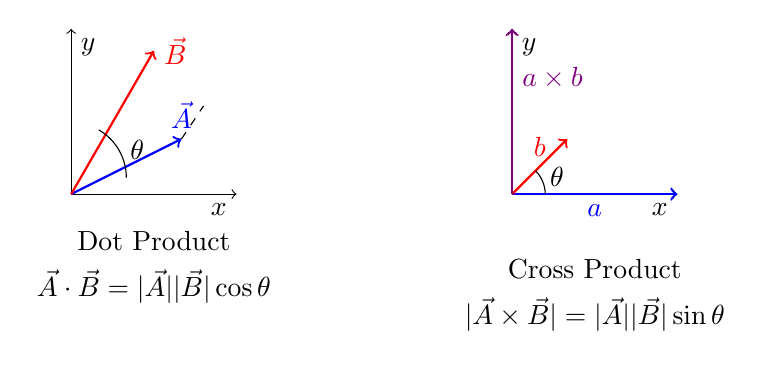
\begin{tikzpicture}[scale=0.7]
		% Axes for dot product
		\begin{scope}[xshift=-4cm]
			\draw[->] (0,0) -- (3,0) node[anchor=north east]{$x$};
			\draw[->] (0,0) -- (0,3) node[anchor=north west]{$y$};
			\draw[->, thick, blue] (0,0) -- (2,1) node[anchor=south]{$\vec{A}$};
			\draw[->, thick, red] (0,0) -- (1.5,2.6) node[anchor=west]{$\vec{B}$};
			\draw[dashed] (2,1) -- (2.4,1.6);
			\draw (1.0,0.3) arc (0:60:1);
			\node at (1.2,0.8) {$\theta$};
			\node[below] at (1.5,-0.5) {Dot Product};
			\node[below] at (1.5,-1.2) {$\vec{A}\cdot\vec{B} = |\vec{A}||\vec{B}|\cos\theta$};
		\end{scope}

		% Axes for cross product
		\begin{scope}[xshift=4cm]
			\draw[->] (0,0,0) -- (3,0,0) node[anchor=north east]{$x$};
			\draw[->] (0,0,0) -- (0,3,0) node[anchor=north west]{$y$};
			\draw[->, thick, blue] (0,0) -- (3,0) node[midway,below]{$a$};
			\draw[->, thick, red] (0,0) -- (1,1) node[midway,above]{$b$};
			\draw[->, thick, blue!50!red] (0,0) -- (0,3) node[pos=0.7,right]{$a\times b$};
			\draw (0.6,0) arc [start angle=0,end angle=45,radius=0.6] node[pos=0.7,right]{$\theta$};
			\node[below] at (1.5,-1) {Cross Product};
			\node[below] at (1.5,-1.7) {$|\vec{A}\times\vec{B}| = |\vec{A}||\vec{B}|\sin\theta$};
		\end{scope}
	\end{tikzpicture}
	\caption{Geometric interpretation of dot and cross products}
\end{figure}

\textbf{Dot product} is just the magnitude of the projection of \(\vec{A}\) onto \(\vec{B}\).

\[
	\vec{A} \times \vec{B} = |\vec{A}| |\vec{B}| \sin \theta \hat{n}
\]

Dot product is the component of $\vec{B}$ along $\vec{A}$. The dot product is a
scalar quantity.

The cross product is a vector that is perpendicular to both \(\vec{A}\) and
\(\vec{B}\) (\(\vec{A} \perp \vec{B}\)). The magnitude of the cross product is
the area of the parallelogram formed by \(\vec{A}\) and \(\vec{B}\). The
direction of the cross product follows the right-hand rule.

\[
	\vec{A} \times \vec{B} = \begin{vmatrix}
		\hat{x} & \hat{y} & \hat{z} \\
		A_x     & A_y     & A_z     \\
		B_x     & B_y     & B_z
	\end{vmatrix}
\]

\subsection{Matrices}
A \textbf{matrix} is a rectangular array of numbers arranged in rows and
columns. Matrices are used to represent linear transformations and solve
systems of linear equations.

\begin{definition}
	A matrix \(A\) with \(m\) rows and \(n\) columns is denoted as \(A \in \mathbb{R}^{m \times n}\). Each element of the matrix is denoted as \(a_{ij}\), where \(i\) is the row index and \(j\) is the column index.
\end{definition}

\begin{equation}
	A = \begin{pmatrix}
		a_{11} & a_{12} & \cdots & a_{1n} \\
		a_{21} & a_{22} & \cdots & a_{2n} \\
		\vdots & \vdots & \ddots & \vdots \\
		a_{m1} & a_{m2} & \cdots & a_{mn}
	\end{pmatrix}
\end{equation}

\textbf{Matrix Addition:} Two matrices \(A\) and \(B\) of the same dimension can be added by adding their corresponding elements.
\begin{equation}
	(A + B)_{ij} = a_{ij} + b_{ij}
\end{equation}

\textbf{Matrix Multiplication:} The product of two matrices \(A \in \mathbb{R}^{m \times n}\) and \(B \in \mathbb{R}^{n \times p}\) is a matrix \(C \in \mathbb{R}^{m \times p}\) where each element is given by the dot product of the corresponding row of \(A\) and column of \(B\).
\begin{equation}
	c_{ij} = \sum_{k=1}^{n} a_{ik} b_{kj}
\end{equation}

\textbf{Identity Matrix:} The identity matrix \(I\) is a square matrix with ones on the diagonal and zeros elsewhere. It acts as the multiplicative identity for matrices.
\begin{equation}
	I = \begin{pmatrix}
		1      & 0      & \cdots & 0      \\
		0      & 1      & \cdots & 0      \\
		\vdots & \vdots & \ddots & \vdots \\
		0      & 0      & \cdots & 1
	\end{pmatrix}
\end{equation}

\textbf{Transpose of a Matrix:} The transpose of a matrix \(A\), denoted \(A^T\), is obtained by swapping its rows and columns.
\begin{equation}
	(A^T)_{ij} = a_{ji}
\end{equation}

\textbf{Determinant of a Matrix:} The determinant is a scalar value that can be computed from the elements of a square matrix and encodes certain properties of the matrix. For a \(2 \times 2\) matrix, the determinant is given by:
\begin{equation}
	\det(A) = \begin{vmatrix}
		a & b \\
		c & d
	\end{vmatrix} = ad - bc
\end{equation}

\textbf{Inverse of a Matrix:} The inverse of a square matrix \(A\), denoted \(A^{-1}\), is the matrix such that \(AA^{-1} = A^{-1}A = I\). A matrix is invertible if and only if its determinant is non-zero.
\begin{equation}
	A^{-1} = \frac{1}{\det(A)} \text{adj}(A)
\end{equation}
where \(\text{adj}(A)\) is the adjugate of \(A\).

\begin{figure}[h]
	\centering
	\begin{tikzpicture}
		\matrix[matrix of math nodes,left delimiter={(},right delimiter={)}] (m) {
			a_{11} & a_{12} & \cdots & a_{1n} \\
			a_{21} & a_{22} & \cdots & a_{2n} \\
			\vdots & \vdots & \ddots & \vdots \\
			a_{m1} & a_{m2} & \cdots & a_{mn} \\
		};
	\end{tikzpicture}
	\caption{Example of a matrix}
\end{figure}

\section{January 13, 2025}
\subsection{Angular Momentum of a Body}
\begin{theorem}
	The angular momentum (relative to the origin) of a body can be found by treating the body as a point mass located at the center of mass (CM) and finding the angular momentum of this point mass relative to the origin, and by then adding on the angular momentum of the body relative to the CM.
\end{theorem}

\begin{proof}
	Let the coordinates of the CM be \( R = (X, Y) \), and let the coordinates of a given point relative to the CM be \( r' = (x', y') \). Then the given point has coordinates \( r = R + r' \). Let the velocity of the CM be \( V \), and let the velocity relative to the CM be \( v' \). Then \( v = V + v' \). Let the body rotate with angular speed \( \omega' \) around the CM. Then \( v' = \omega' r' \).

	The angular momentum relative to the origin is:
	\[
		L = \int (r \times v) \, dm = \int ((R + r') \times (V + v')) \, dm
	\]

	Expanding the cross product:
	\[
		L = \int (R \times V) \, dm + \int (R \times v') \, dm + \int (r' \times V) \, dm + \int (r' \times v') \, dm
	\]

	By the definition of the CM, \( \int r' \, dm = 0 \), so the cross terms
	vanish:
	\[
		L = MR \times V + \int (r' \times v') \, dm
	\]

	Since \( v' = \omega' r' \):
	\[
		L = MR \times V + \left( \int r'^2 \, dm \right) \omega' \hat{z} = MR \times V + I_{CM} \omega' \hat{z}
	\]

	Thus, the angular momentum of the body is the sum of the angular momentum of
	the CM and the angular momentum relative to the CM.
\end{proof}

\subsection{Kinetic Energy of a Body}
\begin{theorem}
	The kinetic energy of a body can be found by treating the body as a point mass located at the CM, and by then adding on the kinetic energy of the body due to the motion relative to the CM.
\end{theorem}

\begin{proof}
	The kinetic energy is:
	\[
		T = \int \frac{1}{2} v^2 \, dm = \int \frac{1}{2} |V + v'|^2 \, dm
	\]

	Expanding the square:
	\[
		T = \int \frac{1}{2} (V^2 + 2V \cdot v' + v'^2) \, dm
	\]

	By the definition of the CM, \( \int v' \, dm = 0 \), so the cross term
	vanishes:
	\[
		T = \frac{1}{2} MV^2 + \int \frac{1}{2} v'^2 \, dm
	\]

	Since \( v' = \omega' r' \):
	\[
		T = \frac{1}{2} MV^2 + \int \frac{1}{2} (\omega' r')^2 \, dm = \frac{1}{2} MV^2 + \frac{1}{2} I_{CM} \omega'^2
	\]

	Thus, the kinetic energy of the body is the sum of the kinetic energy of the CM
	and the kinetic energy relative to the CM.
\end{proof}

\subsection{Parallel-Axis Theorem}
\begin{theorem}
	The moment of inertia of a body about any axis parallel to an axis through the CM is equal to the moment of inertia about the CM axis plus the mass of the body times the square of the distance between the two axes.
\end{theorem}

\begin{proof}
	Consider a body with mass \( M \) and let \( I_{CM} \) be the moment of inertia about an axis through the CM. Let \( R \) be the distance between the CM and the new axis. The moment of inertia about the new axis is:
	\[
		I = \int (r^2 + R^2) \, dm = \int r^2 \, dm + \int R^2 \, dm
	\]

	Since \( R \) is constant:
	\[
		I = I_{CM} + R^2 \int \, dm = I_{CM} + MR^2
	\]

	Thus, the moment of inertia about the new axis is the sum of the moment of
	inertia about the CM axis and \( MR^2 \).
\end{proof}

\subsection{Perpendicular-Axis Theorem}
\begin{theorem}
	For a planar object, the moment of inertia about an axis perpendicular to the plane is equal to the sum of the moments of inertia about two perpendicular axes in the plane.
\end{theorem}

\begin{proof}
	Consider a planar object in the \( x \)-\( y \) plane. The moments of inertia about the \( x \)-axis, \( y \)-axis, and \( z \)-axis are:
	\[
		I_x = \int (y^2 + z^2) \, dm, \quad I_y = \int (z^2 + x^2) \, dm, \quad I_z = \int (x^2 + y^2) \, dm
	\]

	Since the object is planar, \( z = 0 \):
	\[
		I_x = \int y^2 \, dm, \quad I_y = \int x^2 \, dm, \quad I_z = \int (x^2 + y^2) \, dm
	\]

	Thus:
	\[
		I_z = I_x + I_y
	\]

	Therefore, the moment of inertia about the \( z \)-axis is the sum of the
	moments of inertia about the \( x \)-axis and \( y \)-axis.
\end{proof}

\subsection{Non-planar Objects}
In the previous discussion, we restricted the discussion to pancake objects in
the \( x \)-\( y \) plane. However, nearly all the results we derived carry
over to non-planar objects, provided that the axis of rotation is parallel to
the \( z \)-axis, and provided that we are concerned only with \( L_z \), and
not \( L_x \) or \( L_y \). So let’s drop the pancake assumption and run
through the results we obtained above.

First, consider an object rotating around the \( z \)-axis. Let the object have
extension in the \( z \) direction. If we imagine slicing the object into
pancakes parallel to the \( x \)-\( y \) plane, then the equations correctly
give \( L_z \) for each pancake. And since the \( L_z \) of the whole object is
simply the sum of the \( L_z \)'s of all the pancakes, we see that the \( I_z
\) of the whole object is simply the sum of the \( I_z \)'s of all the
pancakes. The difference in the \( z \) values of the pancakes is irrelevant.
Therefore, for any object, we have
\[
	I_z = \int (x^2 + y^2) \, dm, \quad \text{and} \quad L_z = I_z \omega,
\]
where the integration runs over the entire volume of the body. We will
calculate \( I_z \) for many non-planar objects.

Even though the equation gives the \( L_z \) for an arbitrary object, the
analysis is still not completely general because (1) we are restricting the
axis of rotation to be the (fixed) \( z \)-axis, and (2) even with this
restriction, an object outside the \( x \)-\( y \) plane might have nonzero \(
x \) and \( y \) components of \( L \); we found only the \( z \)-component.
This second fact is strange but true. Ponder it for now; we’ll deal with it
later.

As far as the kinetic energy goes, the \( T \) for a non-planar object rotating
around the \( z \)-axis is still given by the same equation, because we can
obtain the total \( T \) by simply adding up the \( T \)'s of each of the
pancake slices.

Also, the equations continue to hold for a non-planar object in the case where
the CM is translating while the object is spinning around it (or more
precisely, spinning around an axis parallel to the \( z \)-axis and passing
through the CM). The velocity \( V \) of the CM can actually point in any
direction, and these two equations will still be valid. But we’ll assume that
all velocities are in the \( x \)-\( y \) plane.

Lastly, the parallel-axis theorem still holds for non-planar objects. But the
perpendicular-axis theorem does not. This is the one instance where we need the
planar assumption.

\subsection{Finding the Center of Mass}
The center of mass has come up repeatedly. For example, when we used the
parallel-axis theorem, we needed to know where the CM was. In some cases, such
as with a stick or a disk, the location is obvious. But in other cases, it
isn’t so clear. So let’s get a little practice calculating the location of the
CM. Depending on whether the mass distribution is discrete or continuous, the
position of the CM is defined by
\[
	R_{CM} = \frac{\sum m_i r_i}{M}, \quad \text{or} \quad R_{CM} = \frac{\int r \, dm}{M},
\]
where \( M \) is the total mass.

\begin{example}
	Find the location of the CM of a hollow hemispherical shell, with uniform mass density and radius \( R \).
\end{example}

\begin{proof}
	By symmetry, the CM is located on the line above the center of the base. So our task reduces to finding the height, \( y_{CM} \). Let the mass density be \( \sigma \). We’ll slice the hemisphere up into horizontal rings, described by the angle \( \theta \) above the horizontal. If the angular thickness of a ring is \( d\theta \), then its mass is
	\[
		dm = \sigma \, dA = \sigma (\text{length}) (\text{width}) = \sigma (2\pi R \cos \theta) (R \, d\theta).
	\]
	All points on the ring have a \( y \) value of \( R \sin \theta \). Therefore,
	\[
		y_{CM} = \frac{1}{M} \int y \, dm = \frac{1}{(2\pi R^2) \sigma} \int_0^{\pi/2} (R \sin \theta) (2\pi R^2 \sigma \cos \theta \, d\theta) = R \int_0^{\pi/2} \sin \theta \cos \theta \, d\theta = \frac{R \sin^2 \theta}{2} \bigg|_0^{\pi/2} = \frac{R}{2}.
	\]
\end{proof}

\subsection{Torque}
We will now show that (under certain conditions, stated below) the rate of
change of angular momentum is equal to a certain quantity, \(\tau\), which we
call the torque. That is, \(\tau = \frac{dL}{dt}\). This is the rotational
analog of our old friend \(F = \frac{dp}{dt}\) involving linear momentum. The
basic idea here is straightforward, but there are two subtle issues. One deals
with internal forces within a collection of particles. The other deals with
origins (the points relative to which the angular momentum is calculated) that
are not fixed. To keep things straight, we’ll prove the general theorem by
dealing with three increasingly complicated situations.

Our derivation of \(\tau = \frac{dL}{dt}\) here holds for completely general
motion; we can take the result and use it in the following chapter, too. If you
wish, you can construct a more specific proof of \(\tau = \frac{dL}{dt}\) for
the special case where the axis of rotation is parallel to the \(z\)-axis. But
since the general proof is no more difficult, we’ll present it here in this
chapter and get it over with.

\subsubsection{Point mass, fixed origin}
Consider a point mass at position \(\vec{r}\) relative to a fixed origin. The
time derivative of the angular momentum, \(L = \vec{r} \times \vec{p}\), is
\[
	\frac{dL}{dt} = \frac{d}{dt} (\vec{r} \times \vec{p}) = \frac{d\vec{r}}{dt} \times \vec{p} + \vec{r} \times \frac{d\vec{p}}{dt} = \vec{v} \times (m\vec{v}) + \vec{r} \times \vec{F} = 0 + \vec{r} \times \vec{F},
\]
where \(\vec{F}\) is the force acting on the particle. This is the same proof
as in Theorem 6.1, except that here we are considering an arbitrary force
instead of a central one. If we define the torque on the particle as
\[
	\tau \equiv \vec{r} \times \vec{F},
\]
then the equation becomes
\[
	\tau = \frac{dL}{dt}.
\]

\subsubsection{Extended mass, fixed origin}
In an extended object, there are internal forces acting on the various pieces
of the object, in addition to whatever external forces exist. For example, the
external force on a given atom in a body might come from gravity, while the
internal forces come from the adjacent atoms. How do we deal with these
different types of forces?

In what follows, we will deal only with internal forces that are central
forces, so that the force between two objects is directed along the line
between them. This is a valid assumption for the pushing and pulling forces
between molecules in a solid. (It isn’t valid, for example, when dealing with
magnetic forces. But we won’t be interested in such things here.) We will
invoke Newton’s third law, which says that the force that particle 1 applies to
particle 2 is equal and opposite to the force that particle 2 applies to
particle 1.

For concreteness, let us assume that we have a collection of \(N\) discrete
particles labeled by the index \(i\). The total angular momentum of the system
is
\[
	L = \sum_{i=1}^{N} \vec{r}_i \times \vec{p}_i.
\]
The force acting on each particle is \(\vec{F}_{\text{ext},i} +
\vec{F}_{\text{int},i} = \frac{d\vec{p}_i}{dt}\). Therefore,
\[
	\frac{dL}{dt} = \frac{d}{dt} \left( \sum_{i} \vec{r}_i \times \vec{p}_i \right) = \sum_{i} \frac{d\vec{r}_i}{dt} \times \vec{p}_i + \sum_{i} \vec{r}_i \times \frac{d\vec{p}_i}{dt} = \sum_{i} \vec{v}_i \times (m_i \vec{v}_i) + \sum_{i} \vec{r}_i \times (\vec{F}_{\text{ext},i} + \vec{F}_{\text{int},i}) = 0 + \sum_{i} \vec{r}_i \times \vec{F}_{\text{ext},i} = \sum_{i} \tau_{\text{ext},i}.
\]
The second-to-last line follows because \(\vec{v}_i \times \vec{v}_i = 0\), and
also because \(\sum_{i} \vec{r}_i \times \vec{F}_{\text{int},i} = 0\), as you
can show in Problem 8. In other words, the internal forces provide no net
torque. This is quite reasonable. It basically says that a rigid object with no
external forces won’t spontaneously start rotating.

Note that the right-hand side involves the total external torque acting on the
body, which may come from forces acting at many different points. Note also
that nowhere did we assume that the particles were rigidly connected to each
other. The equation still holds even if there is relative motion among the
particles.

\subsubsection{Extended mass, non-fixed origin}
Let the position of the origin be \(\vec{r}_0\), and let the positions of the
particles be \(\vec{r}_i\). The vectors \(\vec{r}_0\) and \(\vec{r}_i\) are
measured with respect to a given fixed coordinate system. The total angular
momentum of the system, relative to the (possibly moving) origin \(\vec{r}_0\),
is
\[
	L = \sum_{i} (\vec{r}_i - \vec{r}_0) \times m_i (\dot{\vec{r}}_i - \dot{\vec{r}}_0).
\]
Therefore,
\[
	\frac{dL}{dt} = \frac{d}{dt} \left( \sum_{i} (\vec{r}_i - \vec{r}_0) \times m_i (\dot{\vec{r}}_i - \dot{\vec{r}}_0) \right) = \sum_{i} (\dot{\vec{r}}_i - \dot{\vec{r}}_0) \times m_i (\dot{\vec{r}}_i - \dot{\vec{r}}_0) + \sum_{i} (\vec{r}_i - \vec{r}_0) \times m_i (\ddot{\vec{r}}_i - \ddot{\vec{r}}_0) = 0 + \sum_{i} (\vec{r}_i - \vec{r}_0) \times (\vec{F}_{\text{ext},i} + \vec{F}_{\text{int},i} - m_i \ddot{\vec{r}}_0),
\]
because \(m_i \ddot{\vec{r}}_i\) is the net force (namely
\(\vec{F}_{\text{ext},i} + \vec{F}_{\text{int},i}\)) acting on the \(i\)th
particle. But a quick corollary of Problem 8 is that the term involving
\(\vec{F}_{\text{int},i}\) vanishes (show this). And since \(\sum m_i \vec{r}_i
= M \vec{R}\) (where \(M = \sum m_i\) is the total mass, and \(\vec{R}\) is the
position of the center of mass), we have
\[
	\frac{dL}{dt} = \sum_{i} (\vec{r}_i - \vec{r}_0) \times \vec{F}_{\text{ext},i} - M (\vec{R} - \vec{r}_0) \times \ddot{\vec{r}}_0.
\]
The first term is the external torque, relative to the origin \(\vec{r}_0\).
The second term is something we wish would go away. And indeed, it usually
does. It vanishes if any of the following three conditions is satisfied:
\begin{enumerate}
	\item \(\vec{R} = \vec{r}_0\). That is, the origin is the center of mass.
	\item \(\ddot{\vec{r}}_0 = 0\). That is, the origin is not accelerating.
	\item \((\vec{R} - \vec{r}_0)\) is parallel to \(\ddot{\vec{r}}_0\). This condition is rarely invoked.
\end{enumerate}
If any of these conditions is satisfied, then we are free to write
\[
	\frac{dL}{dt} = \sum_{i} (\vec{r}_i - \vec{r}_0) \times \vec{F}_{\text{ext},i} \equiv \sum_{i} \tau_{\text{ext},i}.
\]
In other words, we can equate the total torque with the rate of change of the
total angular momentum. An immediate corollary of this result is:
\begin{corollary}
	If the total torque on a system is zero, then its angular momentum is conserved. In particular, the angular momentum of an isolated system (one that is subject to no external forces) is conserved.
\end{corollary}

Everything up to this point is valid for arbitrary motion. The particles can be
moving relative to each other, and the various \(L_i\)'s can point in different
directions, etc. But let’s now restrict the motion. In the present chapter, we
are dealing only with cases where \(\hat{L}\) is constant (taken to point in
the \(z\)-direction). Therefore, \(\frac{dL}{dt} = \frac{d(L\hat{L})}{dt} =
\left(\frac{dL}{dt}\right)\hat{L}\). If in addition we consider only rigid
objects (where the relative distances among the particles are fixed) that
undergo pure rotation around a given point, then \(L = I\omega\), which gives
\(\frac{dL}{dt} = I\dot{\omega} \equiv I\alpha\). Taking the magnitude of both
sides of the equation then gives
\[
	\tau = I\alpha.
\]

Invariably, we will calculate angular momentum and torque around either a fixed
point or the center of mass. These are “safe” origins, in the sense that the
equation holds. As long as you vow to always use one of these safe origins, you
can simply apply the equation and not worry much about its derivation.

\begin{example}
	A string wraps around a uniform cylinder of mass \(M\), which rests on a fixed plane. The string passes up over a massless pulley and is connected to a mass \(m\). Assume that the cylinder rolls without slipping on the plane, and that the string is parallel to the plane. What is the acceleration of the mass \(m\)? What is the minimum value of \(M/m\) for which the cylinder accelerates down the plane?
\end{example}

\begin{proof}
	The friction, tension, and gravitational forces are shown in the figure below. Define positive \(a_1\), \(a_2\), and \(\alpha\) as shown. These three accelerations, along with \(T\) and \(F\), are five unknowns. We therefore need to produce five equations. They are:
	\begin{enumerate}
		\item \(F = ma\) on \(m\) \(\Rightarrow T - mg = ma_2\).
		\item \(F = ma\) on \(M\) \(\Rightarrow Mg \sin \theta - T - F = M a_1\).
		\item \(\tau = I\alpha\) on \(M\) (around the center of mass) \(\Rightarrow F R - T R = \left(\frac{MR^2}{2}\right)\alpha\).
		\item Non-slipping condition \(\Rightarrow \alpha = \frac{a_1}{R}\).
		\item Conservation of string \(\Rightarrow a_2 = 2a_1\).
	\end{enumerate}

	A few comments on these equations: The normal force and the gravitational force
	perpendicular to the plane cancel, so we can ignore them. We have picked
	positive \(F\) to point up the plane, but if it happens to point down the plane
	and thereby turn out to be negative, that’s fine (but it won’t); we don’t need
	to worry about which way it really points. In (3), we are using the center of
	mass of the cylinder as our origin, but we can also use a fixed point; see the
	remark below. In (5), we have used the fact that the top of a rolling wheel
	moves twice as fast as the center. This is true because it has the same speed
	relative to the center as the center had relative to the ground.

	We can go about solving these five equations in various ways. Three of the
	equations involve only two variables, so it’s not so bad. (3) and (4) give \(F
	- T = \frac{M a_1}{2}\). Adding this to (2) gives \(Mg \sin \theta - 2T =
	\frac{3M a_1}{2}\). Using (1) to eliminate \(T\), and using (5) to write
	\(a_1\) in terms of \(a_2\), then gives
	\[
		Mg \sin \theta - 2(mg + ma_2) = \frac{3M a_2}{4} \Rightarrow a_2 = \frac{(M \sin \theta - 2m)g}{\frac{3M}{4} + 2m}.
	\]
	And \(a_1 = \frac{a_2}{2}\). We see that \(a_1\) is positive (that is, the
	cylinder rolls down the plane) if \(M/m > \frac{2}{\sin \theta}\).

	\textbf{Remark:} In using \(\tau = \frac{dL}{dt}\), we can also pick a fixed point as our origin, instead of the center of mass. The most sensible point is one located somewhere along the plane. The \(Mg \sin \theta\) force now provides a torque, but the friction does not. The angular momentum of the cylinder with respect to a point on the plane is \(I\omega + MvR\), where the second term comes from the \(L\) due to the object being treated like a point mass at the center of mass. So \(\tau = \frac{dL}{dt}\) becomes \((Mg \sin \theta)R - T(2R) = I\alpha + M a_1 R\). This is simply the sum of the third equation plus \(R\) times the second equation above. We therefore obtain the same result.
\end{proof}

\subsection{Collisions}
In Section 4.7, we looked at collisions involving point particles (or otherwise
nonrotating objects). The fundamental ingredients we used to solve a collision
problem were conservation of momentum and conservation of energy (if the
collision was elastic). With conservation of angular momentum now at our
disposal, we can extend our study of collisions to ones that contain rotating
objects. The additional fact of conservation of \(L\) will be compensated for
by the new degree of freedom for the rotation. Therefore, provided that the
problem is set up properly, we will still have the same number of equations as
unknowns.

In an isolated system, conservation of energy can be used only if the collision
is elastic (by definition). But conservation of angular momentum is similar to
conservation of momentum, in that it can always be used. However, conservation
of \(L\) is a little different from conservation of \(p\), because we have to
pick an origin before we can proceed. In view of the three conditions that are
necessary for Corollary 7.3 to hold, we must pick our origin to be either a
fixed point or the CM of the system (we’ll ignore the third condition, since
it’s rarely used). If we choose some other point, then \(\tau = \frac{dL}{dt}\)
does not hold, so we have no right to claim that \(\frac{dL}{dt}\) equals zero
just because the torque is zero (as it is for an isolated system).

There is, of course, some freedom in choosing an origin from among the legal
possibilities of fixed points or the CM. And since it is generally the case
that one choice is better than the others (in that it makes the calculations
easier), you should take advantage of this freedom.

Let’s do two examples. First, an elastic collision, and then an inelastic one.

\subsubsection{Elastic Collision}
\begin{example}
	A mass \(m\) travels perpendicularly to a stick of mass \(m\) and length \(\ell\), which is initially at rest. At what location should the mass collide elastically with the stick, so that the mass and the center of the stick move with equal speeds after the collision?
\end{example}
\begin{proof}
	Let the initial speed of the mass be \(v_0\). We have three unknowns in the problem, namely the desired distance from the middle of the stick, \(h\); the final (equal) speeds of the stick and the mass, \(v\); and the final angular speed of the stick, \(\omega\). We can solve for these three unknowns by using our three available conservation laws:

	\textbf{Conservation of \(p\):}
	\[
		mv_0 = mv + mv \implies v = \frac{v_0}{2}
	\]

	\textbf{Conservation of \(E\):}
	\[
		\frac{1}{2}mv_0^2 = \frac{1}{2}m\left(\frac{v_0}{2}\right)^2 + \frac{1}{2}m\left(\frac{v_0}{2}\right)^2 + \frac{1}{2}\left(\frac{m\ell^2}{12}\right)\omega^2 \implies \omega = \frac{\sqrt{6}v_0}{\ell}
	\]

	\textbf{Conservation of \(L\):}
	Let’s pick our origin to be the fixed point in space that coincides with the initial location of the center of the stick. Then conservation of \(L\) gives:
	\[
		mv_0h = m\left(\frac{v_0}{2}\right)h + \left(\frac{m\ell^2}{12}\right)\omega + 0
	\]
	The zero here comes from the fact that the CM of the stick moves directly away
	from the origin, so there is no contribution to \(L\) from the first of the two
	parts in Theorem 7.1. Plugging the \(\omega\) from the previous equation into
	this equation gives:
	\[
		\frac{1}{2}mv_0h = \left(\frac{m\ell^2}{12}\right)\left(\frac{\sqrt{6}v_0}{\ell}\right) \implies h = \frac{\ell}{\sqrt{6}}
	\]
\end{proof}

\subsubsection{Inelastic Collision}
\begin{example}
	A mass \(m\) travels at speed \(v_0\) perpendicularly to a stick of mass \(m\) and length \(\ell\), which is initially at rest. The mass collides completely inelastically with the stick at one of its ends, and sticks to it. What is the resulting angular velocity of the system?
\end{example}

\begin{proof}
	The first thing to note is that the CM of the system is \(\frac{\ell}{4}\) from the end. The system will rotate about the CM as the CM moves in a straight line. Conservation of momentum quickly tells us that the speed of the CM is \(\frac{v_0}{2}\). Also, using the parallel-axis theorem, the moment of inertia of the system about the CM is:
	\[
		I_{CM} = I_{\text{stick, CM}} + I_{\text{mass, CM}} = \left(\frac{m\ell^2}{12} + m\left(\frac{\ell}{4}\right)^2\right) + m\left(\frac{\ell}{4}\right)^2 = \frac{5}{24}m\ell^2
	\]

	There are now many ways to proceed, depending on what point we choose as our
	origin.

	\textbf{First method:} Choose the origin to be the fixed point that coincides with the location of the CM right when the collision happens (that is, the point \(\frac{\ell}{4}\) from the end of the stick). Conservation of \(L\) says that the initial \(L\) of the ball must equal the final \(L\) of the system. This gives:
	\[
		mv_0\left(\frac{\ell}{4}\right) = \left(\frac{5}{24}m\ell^2\right)\omega + 0 \implies \omega = \frac{6v_0}{5\ell}
	\]
	The zero here comes from the fact that the CM of the stick moves directly away
	from the origin, so there is no contribution to \(L\) from the first of the two
	parts in Theorem 7.1. Note that we didn’t need to use conservation of \(p\) in
	this method.

	\textbf{Second method:} Choose the origin to be the fixed point that coincides with the initial center of the stick. Then conservation of \(L\) gives:
	\[
		mv_0\left(\frac{\ell}{2}\right) = \left(\frac{5}{24}m\ell^2\right)\omega + (2m)\left(\frac{v_0}{2}\right)\left(\frac{\ell}{4}\right) \implies \omega = \frac{6v_0}{5\ell}
	\]

	\textbf{Third method:} Choose the origin to be the CM of the system. This point moves to the right with speed \(\frac{v_0}{2}\), along the line a distance \(\frac{\ell}{4}\) below the top of the stick. Relative to the CM, the mass \(m\) moves to the right, and the stick moves to the left, both with speed \(\frac{v_0}{2}\). Conservation of \(L\) gives:
	\[
		m\left(\frac{v_0}{2}\right)\left(\frac{\ell}{4}\right) + \left(0 + m\left(\frac{v_0}{2}\right)\left(\frac{\ell}{4}\right)\right) = \left(\frac{5}{24}m\ell^2\right)\omega \implies \omega = \frac{6v_0}{5\ell}
	\]
	The zero here comes from the fact that the stick initially has no \(L\) around
	its center.

	A fourth reasonable choice for the origin is the fixed point that coincides
	with the initial location of the top of the stick. You can work this one out
	for practice.
\end{proof}

\subsection{Angular Impulse}
In Section 4.5.1, we defined the impulse, \(I\), to be the time integral of the
force applied to an object, which is the net change in linear momentum. That
is,
\[
	I \equiv \int_{t_1}^{t_2} F(t) \, dt = \Delta p
\]
We now define the angular impulse, \(I_\theta\), to be the time integral of the
torque applied to an object, which is the net change in angular momentum. That
is,
\[
	I_\theta \equiv \int_{t_1}^{t_2} \tau(t) \, dt = \Delta L
\]
These are just definitions, devoid of any content. The place where the physics
comes in is the following. Consider a situation where \(F(t)\) is always
applied at the same position relative to the origin around which \(\tau(t)\) is
calculated. Let this position be \(R\). Then we have \(\tau(t) = R \times
F(t)\). Plugging this into the previous equation, and taking the constant \(R\)
outside the integral, gives \(I_\theta = R \times I\). That is,
\[
	\Delta L = R \times (\Delta p) \quad \text{(for \(F(t)\) applied at one position)}
\]
This is a very useful result. It deals with the net changes in \(L\) and \(p\),
and not with their changes at any particular instant. Even if \(F\) is changing
in some arbitrary manner as time goes by, so that we have no idea what \(\Delta
p\) and \(\Delta L\) are, we still know that they are related by the previous
equation. Also, note that the derivation of the previous equation was
completely general, so we can apply it in the next chapter, too.

In many cases, we don’t have to worry about the cross product in the previous
equation, because the lever arm \(R\) is perpendicular to the change in
momentum \(\Delta p\). In such cases, we have
\[
	|\Delta L| = R|\Delta p|
\]
Also, in many cases the object starts at rest, so we don’t have to bother with
the \(\Delta\)’s. The following example is a classic application of angular
impulse and the previous equation.

\subsubsection{Striking a Stick}
\begin{example}
	A stick of mass \(m\) and length \(\ell\), initially at rest, is struck with a hammer. The blow is made perpendicular to the stick, at one end. Let the blow occur quickly, so that the stick doesn’t move much while the hammer is in contact. If the CM of the stick ends up moving at speed \(v\), what are the velocities of the ends, right after the blow?
\end{example}
\begin{proof}
	We have no idea exactly what \(F(t)\) looks like, or for how long it is applied, but we do know from the previous equation that \(\Delta L = \left(\frac{\ell}{2}\right)\Delta p\), where \(L\) is calculated relative to the CM (so the lever arm is \(\ell/2\)). Therefore, \(\left(\frac{m\ell^2}{12}\right)\omega = \left(\frac{\ell}{2}\right)mv\). Hence, the final \(v\) and \(\omega\) are related by \(\omega = \frac{6v}{\ell}\).

	The velocities of the ends are obtained by adding (or subtracting) the
	rotational motion to the CM’s translational motion. The rotational velocities
	of the ends are \(\pm\omega\left(\frac{\ell}{2}\right) =
	\pm\left(\frac{6v}{\ell}\right)\left(\frac{\ell}{2}\right) = \pm3v\).
	Therefore, the end that was hit moves with velocity \(v + 3v = 4v\), and the
	other end moves with velocity \(v - 3v = -2v\) (that is, backwards).
\end{proof}

\section{February 18, 2025}
Today, we are starting a new chapter called accelerating frame of reference.
\subsection{Accelerating Frame of Reference}\label[Chapter 10]
Newton's laws hold for both interial and non-inertial frame of references, but for non-intertial frame of references, we have to introduce some `fictious' forces. To be quantitative, we have to spend more time figuring out how the coordinates (and their derivatives) in this accelerating frame of reference are related to the inertial frame of reference.
\subsubsection{Relating the coordinates}
Here, let's consider the following frame of reference. Here we have \(O_1\) is the origin of the inertial frame of reference and \(x_I\) and \(y_I\)
are the axes for this frame, and now let's consider a non-inertial (accelearting) frame of reference, where \(O\) is the origin of the frame and \(x\) and \(y\) are the axes for this frame.
\begin{center}
	\begin{tikzpicture}[>=Stealth]
		% Coordinates
		\coordinate (O1) at (0,0);
		\coordinate (O) at (3,1);
		\coordinate (P) at (4.5,3.5);

		% Axes
		\draw[thick,->] (O1) -- (5,0) node[anchor=north west] {$x_I$};
		\draw[thick,->] (O1) -- (0,4) node[anchor=south east] {$y_I$};
		\draw[thick,->] (O) -- ++(1.5,0.9) node[anchor=north west] {$x$};
		\draw[thick,->] (O) -- ++(-0.5,1.7) node[anchor=south east] {$y$};

		% Vectors
		\draw[very thick,->] (O1) -- (O) node[midway, below right] {$\mathbf{R}$};
		\draw[very thick,->] (O) -- (P) node[midway, right] {$\mathbf{r}$};
		\draw[very thick,->] (O1) -- (P) node[midway, above left] {$\mathbf{r}_I$};

		% Points
		\filldraw (O1) circle (2pt) node[anchor=north east] {$O_I$};
		\filldraw (O) circle (2pt) node[anchor=north east] {$O$};
		\filldraw (P) circle (2pt) node[anchor=south] {$P$};
	\end{tikzpicture}
\end{center}

Let's consider a point \(P\) in these frame of reference, and \(r_I\) is the distance of this point in the inertial frame of reference, but we will write this in the non-inertial frame of reference as following:

\begin{equation}
	\mathbf{r}_I = \mathbf{R} + \mathbf{r}
	\label{eq:10.1}
\end{equation}

But since we haven't defined the system just yet, we will do that now. Here's how the vectors will look in terms of accelerating frames of references:

\begin{equation}
	\begin{aligned}
		\mathbf{R}   & = X \hat{\mathbf{x}}_I + Y \hat{\mathbf{y}}_I + Z \hat{\mathbf{z}}_I       \\
		\mathbf{r}_I & = x_I \hat{\mathbf{x}}_I + y_I \hat{\mathbf{y}}_I + z_I \hat{\mathbf{z}}_I \\
		\mathbf{r}   & = x \hat{\mathbf{x}} + y \hat{\mathbf{y}} + z \hat{\mathbf{z}}
	\end{aligned}
	\label{eq:10.2}
\end{equation}

Now we can write Equation \ref{eq:10.1} in terms of Equation \ref{eq:10.2} as following:

\begin{equation}
	x_I \hat{\mathbf{x}}_I + y_I \hat{\mathbf{y}}_I + z_I \hat{\mathbf{z}}_I = (X \hat{\mathbf{x}}_I + Y \hat{\mathbf{y}}_I + Z \hat{\mathbf{z}}_I) + (x \hat{\mathbf{x}} + y \hat{\mathbf{y}} + z \hat{\mathbf{z}})
	\label{eq:10.3}
\end{equation}
Our goal is to take the time derivative of Eq. \ref{eq:10.1} and interpret the result in an \(\mathbf{F} = m\mathbf{a}\). The second time derivative of \(\mathbf{r_I}\) is the acceleration of the particle in the inertial frame of reference, so according to Newton's second law we have \(\mathbf{F} = m\ddot{\mathbf{r_I}}\). But the second derivative of \(\mathbf{R}\) is in an accelerating frame so we need to account for that as well. Here we can consider writing \(\frac{d^2\mathbf{r}}{dt^2}\) which we can write as \(\frac{d^2\left(\mathbf{r_I} - \mathbf{R}\right)}{dt^2}\) which is not very useful because \(\mathbf{R}\) is accelerating. However, we can write the first part as \(\frac{\delta\mathbf{r}}{dt}\).

To clarify our goal here, we would like to obtain \(\frac{d^2\mathbf{r}}{dt^2}\) in terms of the coordinates in the accelerating frame, because we want to be able to work entirely in terms of these coordinates so that a person in the accelerating frame can write down an \(\mathbf{F} = m\mathbf{a}\) equation in terms of her coordinates only, without having to consider the underlying inertial frame at all. In terms of the inertial frame, \(\frac{d^2\mathbf{r}}{dt^2}\) is simply \(\frac{d^2(\mathbf{r_I} - \mathbf{R})}{dt^2}\), but this isn’t very enlightening by itself.

The following exercise in taking derivatives works for a general vector \(\mathbf{A} = A_x \hat{\mathbf{x}} + A_y \hat{\mathbf{y}} + A_z \hat{\mathbf{z}}\) in the moving frame; it isn’t necessary that it be a position vector. So we’ll work with a general \(\mathbf{A}\) and then set \(\mathbf{A} = \mathbf{r}\) when we’re done. To take \(\frac{d}{dt}\) of \(\mathbf{A} = A_x \hat{\mathbf{x}} + A_y \hat{\mathbf{y}} + A_z \hat{\mathbf{z}}\), we can use the product rule to obtain
\begin{equation}
	\frac{d\mathbf{A}}{dt} = \frac{dA_x}{dt} \hat{\mathbf{x}} + \frac{dA_y}{dt} \hat{\mathbf{y}} + \frac{dA_z}{dt} \hat{\mathbf{z}} + A_x \frac{d\hat{\mathbf{x}}}{dt} + A_y \frac{d\hat{\mathbf{y}}}{dt} + A_z \frac{d\hat{\mathbf{z}}}{dt}.\label{eq:10.4}
\end{equation}
Yes, the product rule works with vectors too. We’re doing nothing more than expanding \((A_x + dA_x)(\hat{\mathbf{x}} + d\hat{\mathbf{x}}) - A_x \hat{\mathbf{x}}\), etc., to first order. Note that although we have expressed the vector \(\mathbf{A}\) in terms of the coordinate axes of the moving frame, the total derivative \(\frac{d\mathbf{A}}{dt}\) is measured with respect to the inertial frame. As mentioned above, the total rate of change of \(\mathbf{A}\) comes from two effects, namely the two groups of terms in the equation above. The first group gives the rate of change of \(\mathbf{A}\), as measured with respect to the moving frame. We’ll denote this quantity by \(\frac{\delta\mathbf{A}}{\delta t}\).

The second group arises because the coordinate axes are moving. In what manner are they moving? We have already extracted the motion of the origin of the accelerating system by introducing the vector \(\mathbf{R}\), so the only thing left is a rotation about some axis \(\boldsymbol{\omega}\) through this origin. The axis \(\boldsymbol{\omega}\) may change with time, but at any instant a unique axis of rotation describes the system. The fact that the axis may change will be relevant in finding the second derivative of \(\mathbf{r}\), but not in finding the first derivative.

We saw that a vector \(\mathbf{B}\) that has fixed length (the coordinate axes here do indeed have fixed length) and that rotates with angular velocity \(\boldsymbol{\omega} \equiv \omega \hat{\boldsymbol{\omega}}\) changes at a rate \(\frac{d\mathbf{B}}{dt} = \boldsymbol{\omega} \times \mathbf{B}\). In particular, \(\frac{d\hat{\mathbf{x}}}{dt} = \boldsymbol{\omega} \times \hat{\mathbf{x}}\), etc. So in the equation above, the \(A_x \frac{d\hat{\mathbf{x}}}{dt}\) term equals \(A_x (\boldsymbol{\omega} \times \hat{\mathbf{x}}) = \boldsymbol{\omega} \times (A_x \hat{\mathbf{x}})\). Likewise for the \(\hat{\mathbf{y}}\) and \(\hat{\mathbf{z}}\) terms. Combining them gives \(\boldsymbol{\omega} \times (A_x \hat{\mathbf{x}} + A_y \hat{\mathbf{y}} + A_z \hat{\mathbf{z}})\), which is just \(\boldsymbol{\omega} \times \mathbf{A}\). Therefore, the equation becomes
\begin{equation}
	\frac{d\mathbf{A}}{dt} = \frac{\delta\mathbf{A}}{\delta t} + \boldsymbol{\omega} \times \mathbf{A}.\label{eq:10.5}
\end{equation}
We still have to take one more time derivative. Using the product rule, the time derivative of the equation above is
\begin{equation}
	\frac{d^2\mathbf{A}}{dt^2} = \frac{d}{dt} \left( \frac{\delta\mathbf{A}}{\delta t} \right) + \frac{d\boldsymbol{\omega}}{dt} \times \mathbf{A} + \boldsymbol{\omega} \times \frac{d\mathbf{A}}{dt}.\label{eq:10.6}
\end{equation}
Applying the previous result to the first term on the right (with \(\frac{\delta\mathbf{A}}{\delta t}\) in place of \(\mathbf{A}\)), and plugging the previous result into the third term, gives
\begin{equation}
	\frac{d^2\mathbf{A}}{dt^2} = \frac{\delta^2\mathbf{A}}{\delta t^2} + \boldsymbol{\omega} \times \frac{\delta\mathbf{A}}{\delta t} + \frac{d\boldsymbol{\omega}}{dt} \times \mathbf{A} + \boldsymbol{\omega} \times \left( \frac{\delta\mathbf{A}}{\delta t} + \boldsymbol{\omega} \times \mathbf{A} \right).\label{eq:10.7}
\end{equation}
Simplifying, we get
\begin{equation}
	\frac{d^2\mathbf{A}}{dt^2} = \frac{\delta^2\mathbf{A}}{\delta t^2} + \boldsymbol{\omega} \times (\boldsymbol{\omega} \times \mathbf{A}) + 2\boldsymbol{\omega} \times \frac{\delta\mathbf{A}}{\delta t} + \frac{d\boldsymbol{\omega}}{dt} \times \mathbf{A}.\label{eq:10.8}
\end{equation}
At this point we will set \(\mathbf{A} = \mathbf{r}\), which gives
\begin{equation}
	\frac{d^2\mathbf{r}}{dt^2} = \mathbf{a} + \boldsymbol{\omega} \times (\boldsymbol{\omega} \times \mathbf{r}) + 2\boldsymbol{\omega} \times \mathbf{v} + \frac{d\boldsymbol{\omega}}{dt} \times \mathbf{r},\label{eq:10.8}
\end{equation}
where \(\mathbf{r}\), \(\mathbf{v} \equiv \frac{\delta\mathbf{r}}{\delta t}\), and \(\mathbf{a} \equiv \frac{\delta^2\mathbf{r}}{\delta t^2}\) are the position, velocity, and acceleration of the particle, as measured with respect to the accelerating frame. In other words, if the accelerating frame is enclosed in a windowless box, and if a person inside the box paints a coordinate grid on the floor, then she can (assuming that she has a clock at her disposal) measure \(\mathbf{r}\), \(\mathbf{v}\), and \(\mathbf{a}\) without caring at all about what is going on in the outside world.

You might be concerned that the \(\mathbf{r}\), \(\mathbf{v}\), and \(\mathbf{a}\) on the right-hand side of the equation are measured by someone in the rotating frame, whereas the \(\frac{d^2\mathbf{r}}{dt^2}\) on the left-hand side is measured by someone in the inertial frame. But this apparent discrepancy is a nonissue, because the equation is a statement about vectors, and these vectors have an existence that is independent of the coordinate system that is used to describe them. For example, the vector \(\mathbf{a}\) points in a certain direction (say, toward the distant star Sirius) and has a certain magnitude, independent of whoever chooses to describe it with whatever coordinates.

\subsection{Fictious Force}
From Eq.(\ref{eq:10.1}) we already have
\begin{equation}
	\frac{d^2\mathbf{r}}{dt^2} = \frac{d^2\mathbf{r_I}}{dt^2} - \frac{d^2\mathbf{R}}{dt^2}
	\label{10.9}
\end{equation}
Now, we can equate that to the Eq.(\ref{eq:10.8}) and multiply by the mass \(m\) and we realize that it's simply force \(\mathbf{F}\) acting on the particle and solging for \(m\mathbf{a}\) we get the following:

\begin{equation}
	\begin{aligned}
		m\mathbf{a} & = \mathbf{F} - m\frac{d^2\mathbf{R}}{dt^2} + m\boldsymbol{\omega} \times (\boldsymbol{\omega} \times \mathbf{r}) + 2m\boldsymbol{\omega} \times \mathbf{v} + m\frac{d\boldsymbol{\omega}}{dt} \times \mathbf{r} \\
		            & \equiv \mathbf{F} + \mathbf{F_{translational}} + \mathbf{F_{centrifuga}} + \mathbf{F_{Coriolis}} + \mathbf{F_{azimuthal}}
	\end{aligned}\label{eq:10.10}
\end{equation}
That means we can \vocab{fictious forces} as following:
\begin{equation}
	\begin{aligned}
		\mathbf{F_{translational}} & \equiv -m\frac{d^2\mathbf{R}}{dt^2}                                        \\
		\mathbf{F_{centrifuga}}    & \equiv m\boldsymbol{\omega} \times (\boldsymbol{\omega} \times \mathbf{r}) \\
		\mathbf{F_{Coriolis}}      & \equiv 2m\boldsymbol{\omega} \times \mathbf{v}                             \\
		\mathbf{F_{azimuthal}}     & \equiv m\frac{d\boldsymbol{\omega}}{dt} \times \mathbf{r}
	\end{aligned}\label{eq:10.11}
\end{equation}


\section{Februrary 19, 2025}
\begin{example}
	A stick rotates with \(\vec{\omega} = \omega \hat{z}\) and one end fixed to a pivot. The little \(dm\) a distance \(s\) from the pivot experiences a centrifugal force \(d\vec{F}_{\text{cent}} = ?\)
\end{example}

\begin{solution}

\end{solution}
\begin{example}
	A stick rotates with \(\vec{\omega} = \omega \hat{z}\) and one end fixed to a pivot. If the centrifugal force on an element \(dm\) is \(d\vec{F}_{\text{cent}} = dm \omega^2 s \sin\phi \hat{r}\), then the contribution to the torque around the pivot point (top end of the stick) is:
\end{example}
\begin{solution}
	Here, the \(d\vec{F}_{\text{cent}} = s \, dm \, \omega^2 \sin\phi \, \hat{r}\) and \(\hat{r} = \sin\phi \, \hat{r} - \cos\phi \, \hat{z}\).
\end{solution}



\begin{example}
	On Earth at the equator \((R\sim 6400 km)\), how big is the centrifugal force, expressed as a fraction of gravity, i.e.  \(F_{cent}/(mg)\approx\)?
\end{example}
\begin{solution}
	Here, the radius, \(r = 6.4 \times 10^5\) m, and \(\omega = \frac{2\pi}{24 \times 60 \times 60}\), and we plug that into the formula \[\frac{F_{cent}}{mg} = \frac{m\omega^2 r}{mg} = \frac{\omega^2 r}{g} = \frac{\left(\frac{2\pi}{24 \times 60 \times 60}\right)^2 \cdot (6.4 \times 10^5)}{9.8} \sim 0.003\]
\end{solution}



%\section{February 21, 2025}
%\section{February 24, 2025}
%\section{February 26, 2025}
%\section{February 28, 2025}
%\section{March 3, 2025}
%\section{March 5, 2025}
%\section{March 7, 2025}
%\section{March 17, 2025}
%\section{March 19, 2025}
%\section{March 21, 2025}
%\section{March 24, 2025}
%\section{March 26, 2025}
%\section{March 28, 2025}
%\section{March 31, 2025}
%\section{April 2, 2025}
%\section{April 4, 2025}
%\section{April 7, 2025}
%\section{April 9, 2025}
%\section{April 11, 2025}
%\section{April 14, 2025}
%\section{April 16, 2025}
%\section{April 18, 2025}
%\section{April 21, 2025}
%\section{April 23, 2025}
%\section{April 25, 2025}
%\section{April 28, 2025}

\end{document}
